
\documentclass{article}
\usepackage{multirow}
\usepackage[table]{xcolor}
\usepackage{tikz}
\usepackage{tgheros}
% The default underscores are very short :/
\renewcommand{\_}[0]{\rule{5pt}{1pt}}
% Use sans-serif font by default.
\renewcommand{\familydefault}{\sfdefault}
% Convenience commands for table styling.
\newcommand{\upr}[1]{\raisebox{0.5em}[0.5em][0em]{#1}}
\newcommand{\upri}[1]{\upr{\textit{#1}}}
\newcommand{\uprb}[1]{\upr{\textbf{#1}}}
% Styling for 'N/A' cells.
\newcommand{\tcna}[1]{\cellcolor[HTML]{CCCCCC} \textit{#1}}
\newcommand{\tcnaup}[1]{\tcna{\upri{#1}}}
% Styling for peripheral cells.
\newcommand{\tcpA}[1]{\cellcolor[HTML]{2EF43F} #1}
\newcommand{\tcpAup}[1]{\upr{\cellcolor[HTML]{2EF43F} #1}}
\newcommand{\tcpB}[1]{\cellcolor[HTML]{EF7CD8} #1}
\newcommand{\tcpBup}[1]{\upr{\cellcolor[HTML]{EF7CD8} #1}}
\newcommand{\tcpC}[1]{\cellcolor[HTML]{1DABE2} #1}
\newcommand{\tcpCup}[1]{\upr{\cellcolor[HTML]{1DABE2} #1}}
\newcommand{\tcpD}[1]{\cellcolor[HTML]{E83030} #1}
\newcommand{\tcpDup}[1]{\upr{\cellcolor[HTML]{E83030} #1}}
\newcommand{\tcpE}[1]{\cellcolor[HTML]{C8EA1E} #1}
\newcommand{\tcpEup}[1]{\upr{\cellcolor[HTML]{C8EA1E} #1}}
\newcommand{\tcpF}[1]{\cellcolor[HTML]{F2840E} #1}
\newcommand{\tcpFup}[1]{\upr{\cellcolor[HTML]{F2840E} #1}}
% Set page dimensions.
\usepackage[paperwidth=150em, paperheight=35em,
            top=5em, bottom=0em, left=0em, right=0em]{geometry}

\begin{document}
\pagenumbering{gobble}

\begin{table}[h!]
  \begin{center}
    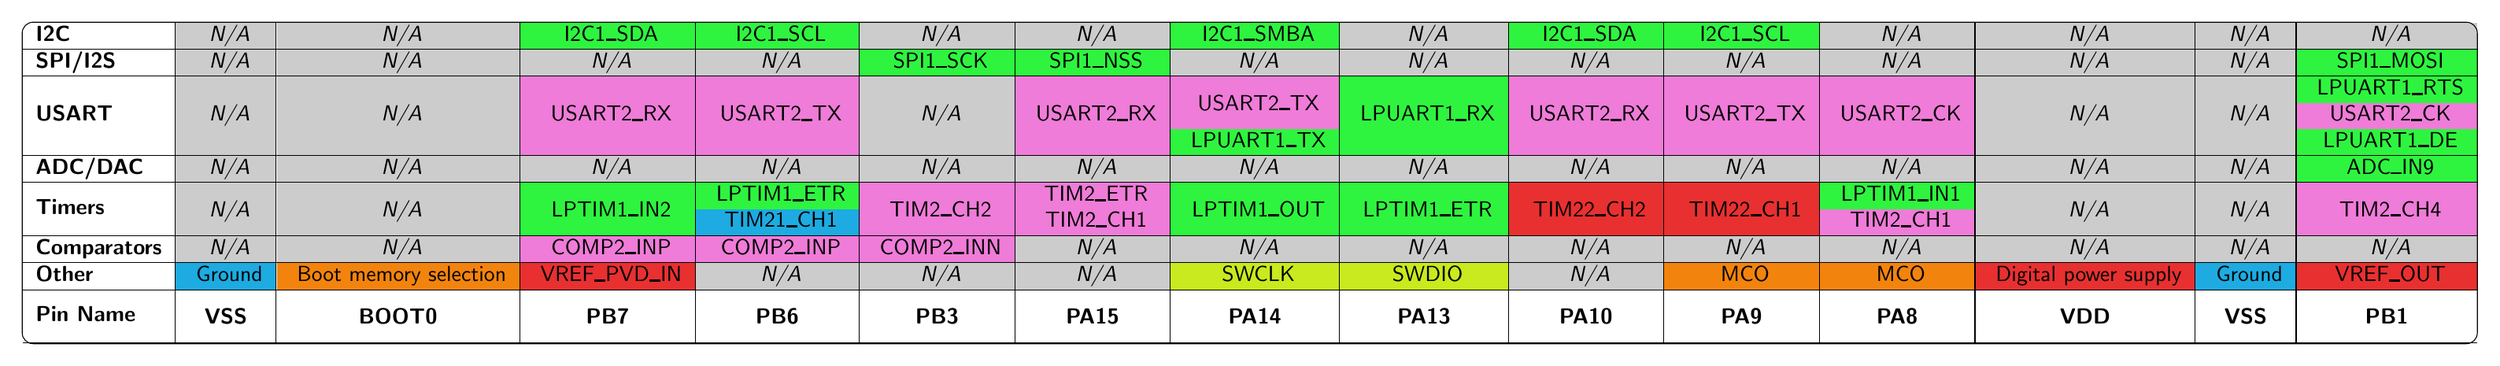
\begin{tikzpicture}
      \node (table) [inner sep=0pt] {
        \begin{tabular}{l|c|c|c|c|c|c|c|c|c|c|c|c|c|c}
\textbf{I2C}
& \tcna{N/A} & \tcna{N/A} & \tcpA{I2C1\_SDA} & \tcpA{I2C1\_SCL} & \tcna{N/A} & \tcna{N/A} & \tcpA{I2C1\_SMBA} & \tcna{N/A} & \tcpA{I2C1\_SDA} & \tcpA{I2C1\_SCL} & \tcna{N/A} & \tcna{N/A} & \tcna{N/A} & \tcna{N/A}  \\
\hline
\textbf{SPI/I2S}
& \tcna{N/A} & \tcna{N/A} & \tcna{N/A} & \tcna{N/A} & \tcpA{SPI1\_SCK} & \tcpA{SPI1\_NSS} & \tcna{N/A} & \tcna{N/A} & \tcna{N/A} & \tcna{N/A} & \tcna{N/A} & \tcna{N/A} & \tcna{N/A} & \tcpA{SPI1\_MOSI}  \\
\hline
\multirow{3}{*}{\textbf{USART}}& \tcna{} & \tcna{} & \tcpB{} & \tcpB{} & \tcna{} & \tcpB{} & \tcpB{} & \tcpA{} & \tcpB{} & \tcpB{} & \tcpB{} & \tcna{} & \tcna{} & \tcpA{LPUART1\_RTS}  \\
& \tcna{N/A} & \tcna{N/A} & \tcpB{USART2\_RX} & \tcpB{USART2\_TX} & \tcna{N/A} & \tcpB{USART2\_RX} & \tcpBup{USART2\_TX} & \tcpA{LPUART1\_RX} & \tcpB{USART2\_RX} & \tcpB{USART2\_TX} & \tcpB{USART2\_CK} & \tcna{N/A} & \tcna{N/A} & \tcpB{USART2\_CK}  \\
& \tcna{} & \tcna{} & \tcpB{} & \tcpB{} & \tcna{} & \tcpB{} & \tcpA{LPUART1\_TX} & \tcpA{} & \tcpB{} & \tcpB{} & \tcpB{} & \tcna{} & \tcna{} & \tcpA{LPUART1\_DE}  \\
\hline
\textbf{ADC/DAC}
& \tcna{N/A} & \tcna{N/A} & \tcna{N/A} & \tcna{N/A} & \tcna{N/A} & \tcna{N/A} & \tcna{N/A} & \tcna{N/A} & \tcna{N/A} & \tcna{N/A} & \tcna{N/A} & \tcna{N/A} & \tcna{N/A} & \tcpA{ADC\_IN9}  \\
\hline
\multirow{2}{*}{\textbf{Timers}}& \tcna{} & \tcna{} & \tcpA{} & \tcpA{LPTIM1\_ETR} & \tcpB{} & \tcpB{TIM2\_ETR} & \tcpA{} & \tcpA{} & \tcpD{} & \tcpD{} & \tcpA{LPTIM1\_IN1} & \tcna{} & \tcna{} & \tcpB{}  \\
& \tcnaup{N/A} & \tcnaup{N/A} & \tcpAup{LPTIM1\_IN2} & \tcpC{TIM21\_CH1} & \tcpBup{TIM2\_CH2} & \tcpB{TIM2\_CH1} & \tcpAup{LPTIM1\_OUT} & \tcpAup{LPTIM1\_ETR} & \tcpDup{TIM22\_CH2} & \tcpDup{TIM22\_CH1} & \tcpB{TIM2\_CH1} & \tcnaup{N/A} & \tcnaup{N/A} & \tcpBup{TIM2\_CH4}  \\
\hline
\textbf{Comparators}
& \tcna{N/A} & \tcna{N/A} & \tcpB{COMP2\_INP} & \tcpB{COMP2\_INP} & \tcpB{COMP2\_INN} & \tcna{N/A} & \tcna{N/A} & \tcna{N/A} & \tcna{N/A} & \tcna{N/A} & \tcna{N/A} & \tcna{N/A} & \tcna{N/A} & \tcna{N/A}  \\
\hline
\textbf{Other}
& \tcpC{Ground} & \tcpF{Boot memory selection} & \tcpD{VREF\_PVD\_IN} & \tcna{N/A} & \tcna{N/A} & \tcna{N/A} & \tcpE{SWCLK} & \tcpE{SWDIO} & \tcna{N/A} & \tcpF{MCO} & \tcpF{MCO} & \tcpD{Digital power supply} & \tcpC{Ground} & \tcpD{VREF\_OUT}  \\
\hline
\multirow{2}{*}{\textbf{Pin Name}} & & & & & & & & & & & & & & \\
& \uprb{VSS}& \uprb{BOOT0}& \uprb{PB7}& \uprb{PB6}& \uprb{PB3}& \uprb{PA15}& \uprb{PA14}& \uprb{PA13}& \uprb{PA10}& \uprb{PA9}& \uprb{PA8}& \uprb{VDD}& \uprb{VSS}& \uprb{PB1}\\
\hline

        \end{tabular}
      };
      \draw [rounded corners=0.5em]
        (table.north west) rectangle (table.south east);
    \end{tikzpicture}
  \end{center}
\end{table}

\end{document}
